%%%%%%%%%%%%%%%%%%%%%%%%%%%%%%%%%%%%%%%%%%%%%%%%%%%%%%%%%%%%%%%%%%%%%%%%%%%%%%%%
% VPIC Gordon Bell submission 2008
%
% $LastChangedRevision$
% $LastChangedDate$
% $LastChangedBy$
%
%%%%%%%%%%%%%%%%%%%%%%%%%%%%%%%%%%%%%%%%%%%%%%%%%%%%%%%%%%%%%%%%%%%%%%%%%%%%%%%%
\documentclass[letter,10pt]{article}

%%%%%%%%%%%%%%%%%%%%%%%%%%%%%%%%%%%%%%%%%%%%%%%%%%%%%%%%%%%%%%%%%%%%%%%%%%%%%%%%
% packages
%%%%%%%%%%%%%%%%%%%%%%%%%%%%%%%%%%%%%%%%%%%%%%%%%%%%%%%%%%%%%%%%%%%%%%%%%%%%%%%%
\usepackage{amsmath}
\usepackage{color}
\usepackage{latexmake}
\usepackage{setspace}
\doublespacing


%%%%%%%%%%%%%%%%%%%%%%%%%%%%%%%%%%%%%%%%%%%%%%%%%%%%%%%%%%%%%%%%%%%%%%%%%%%%%%%%
% macaros cribbed from Kevin's PoP paper
%%%%%%%%%%%%%%%%%%%%%%%%%%%%%%%%%%%%%%%%%%%%%%%%%%%%%%%%%%%%%%%%%%%%%%%%%%%%%%%%
\newcommand{\eps}{\varepsilon}
\newcommand{\vecr}{\vec{r}}
\newcommand{\vecu}{\vec{u}}
\newcommand{\vecJ}{\vec{J}}
\newcommand{\vecP}{\vec{P}}
\newcommand{\vecE}{\vec{E}}
\newcommand{\vecB}{\vec{B}}
\newcommand{\tensT}{\mathbf{T}}
\newcommand{\tensP}{\mathbf{\Pi}}
\newcommand{\tensS}{\mathbf{\Xi}}
\newcommand{\EN}{\mathcal{E}}
\newcommand{\op}{\mathcal{L}}

\newcommand{\Expect}[1]{\left< #1 \right>}
\newcommand{\Deriv}[2]{d_{#2}#1}
\newcommand{\PDeriv}[2]{\partial_{#2}#1}

\newcommand{\DotP}[2]{#1 \cdot #2}
\newcommand{\CrossP}[2]{#1 \times #2}

\newcommand{\Grad}[1]{\nabla #1}
\newcommand{\Div}[1]{\nabla \cdot #1}
\newcommand{\Curl}[1]{\nabla \times #1}

\newcommand{\Gradu}[1]{\nabla_{\vecu} #1}
\newcommand{\Divu}[1]{\nabla_{\vecu} \cdot #1}
\newcommand{\Curlu}[1]{\nabla_{\vecu} \times #1}

\newcommand{\eq}[1]{(\ref{eq:#1})}
\newcommand{\tbl}[1]{Table \ref{tbl:#1}}
\newcommand{\fig}[1]{Figure \ref{fig:#1}}

%%%%%%%%%%%%%%%%%%%%%%%%%%%%%%%%%%%%%%%%%%%%%%%%%%%%%%%%%%%%%%%%%%%%%%%%%%%%%%%%
% Brian needs macaros too 
%%%%%%%%%%%%%%%%%%%%%%%%%%%%%%%%%%%%%%%%%%%%%%%%%%%%%%%%%%%%%%%%%%%%%%%%%%%%%%%%
\newcommand{\abinitio} {\textit{ab initio}}
\newcommand{\lde}      {\lambda_{\mathrm{De}}}
\newcommand{\wpe}      {\omega_{\mathrm{pe}}}

%%%%%%%%%%%%%%%%%%%%%%%%%%%%%%%%%%%%%%%%%%%%%%%%%%%%%%%%%%%%%%%%%%%%%%%%%%%%%%%%
% add to document dimensions
% fudge if we need to add more space
%%%%%%%%%%%%%%%%%%%%%%%%%%%%%%%%%%%%%%%%%%%%%%%%%%%%%%%%%%%%%%%%%%%%%%%%%%%%%%%%
\addtolength{\topmargin}{-2cm}
\addtolength{\textheight}{3cm}
\addtolength{\oddsidemargin}{-2.25cm}
\addtolength{\evensidemargin}{-2.25cm}
\addtolength{\textwidth}{4.5cm}

%%%%%%%%%%%%%%%%%%%%%%%%%%%%%%%%%%%%%%%%%%%%%%%%%%%%%%%%%%%%%%%%%%%%%%%%%%%%%%%%
% article information
%%%%%%%%%%%%%%%%%%%%%%%%%%%%%%%%%%%%%%%%%%%%%%%%%%%%%%%%%%%%%%%%%%%%%%%%%%%%%%%%
\title{0.4 PFlop/s Trillion-Particle Particle-in-Cell Modeling of Laser Plasma Interactions on Roadrunner}
\author{%
B. J. Albright\thanks{Applied Physics Division (X-1-PTA Plasma Theory and Applications), Los Alamos National Laboratory, Los Alamos, NM 87544, Email: \emph{balbright@lanl.gov}} \and%
%
K. Barker\thanks{Computer, Computational, and Statistical Sciences Division (CCS-1 Computer Science on High Performance Computing), Los Alamos National Laboratory, Los Alamos, NM 87544, Email: \emph{kjbarker@lanl.gov}} \and%
%
B. Bergen\thanks{Computer, Computational, and Statistical Sciences Division (CCS-2 Computational Physics), Los Alamos National Laboratory, Los Alamos, NM 87544, Email: \emph{bergen@lanl.gov}} \and%
%
K. J. Bowers\thanks{D.E. Shaw Research LLC, 120 W 45th Street, 39th Floor, New York, NY 10036, Email: \emph{kevin.j.bowers@gmail.com}} \and%
%
D. Kerbyson\thanks{Computer, Computational, and Statistical Sciences Division (CCS-1 Computer Science on High Performance Computing), Los Alamos National Laboratory, Los Alamos, NM 87544, Email: \emph{djk@lanl.gov}} \and%
%
L. Yin\thanks{Applied Physics Division (X-1-PTA Plasma Theory and Applications), Los Alamos National Laboratory, Los Alamos, NM 87544, Email: \emph{lyin@lanl.gov}}}
\date{\today}

% if we have assessment, then we need to include CCS-1 types, no? 

%%%%%%%%%%%%%%%%%%%%%%%%%%%%%%%%%%%%%%%%%%%%%%%%%%%%%%%%%%%%%%%%%%%%%%%%%%%%%%%%
% begin document
%%%%%%%%%%%%%%%%%%%%%%%%%%%%%%%%%%%%%%%%%%%%%%%%%%%%%%%%%%%%%%%%%%%%%%%%%%%%%%%%
\begin{document}

%%%%%%%%%%%%%%%%%%%%%%%%%%%%%%%%%%%%%%%%%%%%%%%%%%%%%%%%%%%%%%%%%%%%%%%%%%%%%%%%
% title
%%%%%%%%%%%%%%%%%%%%%%%%%%%%%%%%%%%%%%%%%%%%%%%%%%%%%%%%%%%%%%%%%%%%%%%%%%%%%%%%
\maketitle
\thispagestyle{empty}

%%%%%%%%%%%%%%%%%%%%%%%%%%%%%%%%%%%%%%%%%%%%%%%%%%%%%%%%%%%%%%%%%%%%%%%%%%%%%%%%
% abstract
%%%%%%%%%%%%%%%%%%%%%%%%%%%%%%%%%%%%%%%%%%%%%%%%%%%%%%%%%%%%%%%%%%%%%%%%%%%%%%%%
\begin{singlespace}
\begin{abstract}
We demonstrate the outstanding performance and scalability of the VPIC 
kinetic plasma modeling code on the heterogeneous IBM Roadrunner 
supercomputer at Los Alamos National Laboratory.  VPIC is a three-
dimensional, relativistic, electromagnetic, particle-in-cell code that 
self-consistently evolves a kinetic plasma.  VPIC simulations of laser 
plasma interaction (LPI) have been conducted at unprecedented fidelity 
and scale ---one trillion simulation macro particles on 125 million 
computational cells-- to accurately model the plasma environment 
inside a laser-driven hohlraum in an inertial confinement fusion 
experiment.   Sustained performance of approximately 0.4~Pflop/s was 
achieved.  This capability opens up the exciting possibility of using 
VPIC to model, in a first-principles manner, a problem that threatens 
the success of the multi-billion dollar DOE/NNSA National Ignition Facility.  
\end{abstract}
\end{singlespace}

%%%%%%%%%%%%%%%%%%%%%%%%%%%%%%%%%%%%%%%%%%%%%%%%%%%%%%%%%%%%%%%%%%%%%%%%%%%%%%%%
% add break after title page
%%%%%%%%%%%%%%%%%%%%%%%%%%%%%%%%%%%%%%%%%%%%%%%%%%%%%%%%%%%%%%%%%%%%%%%%%%%%%%%%
\pagebreak

%%%%%%%%%%%%%%%%%%%%%%%%%%%%%%%%%%%%%%%%%%%%%%%%%%%%%%%%%%%%%%%%%%%%%%%%%%%%%%%%
% Introduction
%%%%%%%%%%%%%%%%%%%%%%%%%%%%%%%%%%%%%%%%%%%%%%%%%%%%%%%%%%%%%%%%%%%%%%%%%%%%%%%%
\section*{Introduction}

%%%%%%%%%%%%%%%%%%%%%%%%%%%%%%%%%%%%%%%%%%%%%%%%%%%%%%%%%%%%%%%%%%%%%%%%%%%%%%%%
% Architecture
%%%%%%%%%%%%%%%%%%%%%%%%%%%%%%%%%%%%%%%%%%%%%%%%%%%%%%%%%%%%%%%%%%%%%%%%%%%%%%%%
\section*{RoadRunner system architecture}

\begin{figure}
    \begin{center}
    \scalebox{0.3}{\input{system.pstex_t}}
    \caption{RoadRunner System Overview}
    \label{fig:system}
    \end{center}
\end{figure}

The RoadRunner supercomputer, shown in Figure \ref{fig:system},
is a hybrid, petascale system to be deployed at Los Alamos National
Laboratory in 2008.  The system is a first-of-its-kind, heterogeneous
cluster-of-clusters that utilizes a combination of 6,912, 1.8 GHz,
dual-socket, dual-core AMD Opteron \emph{host} processors with 12,960,
3.2 GHz, IBM \emph{PowerXCell 8I accelerator} chips also known as the
Cell \emph{extended Double Precision (eDP)} processor (throughout the
rest of this paper we will refer to this chip as the Cell eDP processor).
Each Cell eDP processor is capable of performing 102.4 Gflop/s
double-precision (204.8 GFlop/s single-precision), for a total
theoretical peak performance of $\sim$1.3 Pflop/s\footnote{The Opteron
base system has a theoretical peak performance of $\sim$50 Tflop/s that
is not included in this figure.}.
The RoadRunner supercomputer will be the first machine to achieve a
sustained petaflop on the LINPACK benchmark used in ranking the
fastest supercomputers in the world for the TOP500 list \cite{top500}.

\subsection*{Connected Unit}

A Connected Unit (CU) is made up of 180 \emph{Triblade}, compute
nodes and 12 I/O nodes linked by a first-stage, 288-port Voltaire
Infiniband $4x$ DDR switch.  Using a top-down description, the
system is comprised of 18 CUs connected via eight, second-stage,
288-port Voltaire Infiniband $4x$ DDR switches.  This allows for
twelve links per CU to each of the eight switches, with 192 ports
\emph{in} and 96 ports \emph{up}, creating a 2-to-1 over-subscribed,
fat-tree network topology.

A Connected Unit is a powerful cluster in 
its own right, with a theoretical peak performance of
$\sim$74 Tflop/s.  A single CU of RoadRunner would rank in the
top 20 on the current (November 2007) TOP500 list.

\begin{figure}
    \begin{center}
    \scalebox{0.2}{\input{triblade.pstex_t}}
    \caption{Triblade Compute Node}
    \label{fig:triblade}
    \end{center}
\end{figure}

\subsection*{Triblade}

A Triblade compute node, Figure \ref{fig:triblade}, actually integrates
four physical blades: one IBM LS21, dual-socket Opteron blade, one
expansion blade, and two IBM QS22 Cell blades containing the new
Cell eDP processors.  The expansion blade connects the two QS22s to
the LS21 via four PCI-e $x8$ links and provides the node's
ConnectX IB $4x$ DDR link to the rest of the CU cluster.
Each PCI-e $x8$ link logically connects an Opteron core to a
Cell eDP processor ---there is a one-to-one relationship between
Opteron cores and eDP processors-- with a theoretical bandwidth
of 2 GB/s.  Triblades are completely diskless, running from RAM disks
with NFS and Panasas \cite{panasas} to the LS21 only.

The LS21 blade incorporates two dual-core AMD Opteron processors
running at 1.8 GHz with 4 GB RAM per core.  Each LS21 has a
theoretical peak of 14.4 Gflop/s in double precision.

Each QS22 blade has two Cell eDP processors running at 3.2 GHz
with 8 GB RAM so that each Cell chip has 4 GB RAM.  The two QS22
blades have an aggregate theoretical peak performance of
409.6 Gflop/s in double precision.

In total, each Triblade has 32 GB RAM, with 16 GB RAM on the
LS21 blade and 16 GB RAM each per QS22 blade, so that each
logical processor in a compute node has 4 GB RAM.  The total
theoretical peak performance per Triblade is 424 Gflop/s in
double precision.  The full RoadRunner machine has a total of
3240 Triblade compute nodes.

\subsection*{Cell Broadband Engine Architecture (CBEA)}

%\begin{figure}
%    \begin{center}
%    \scalebox{0.5}{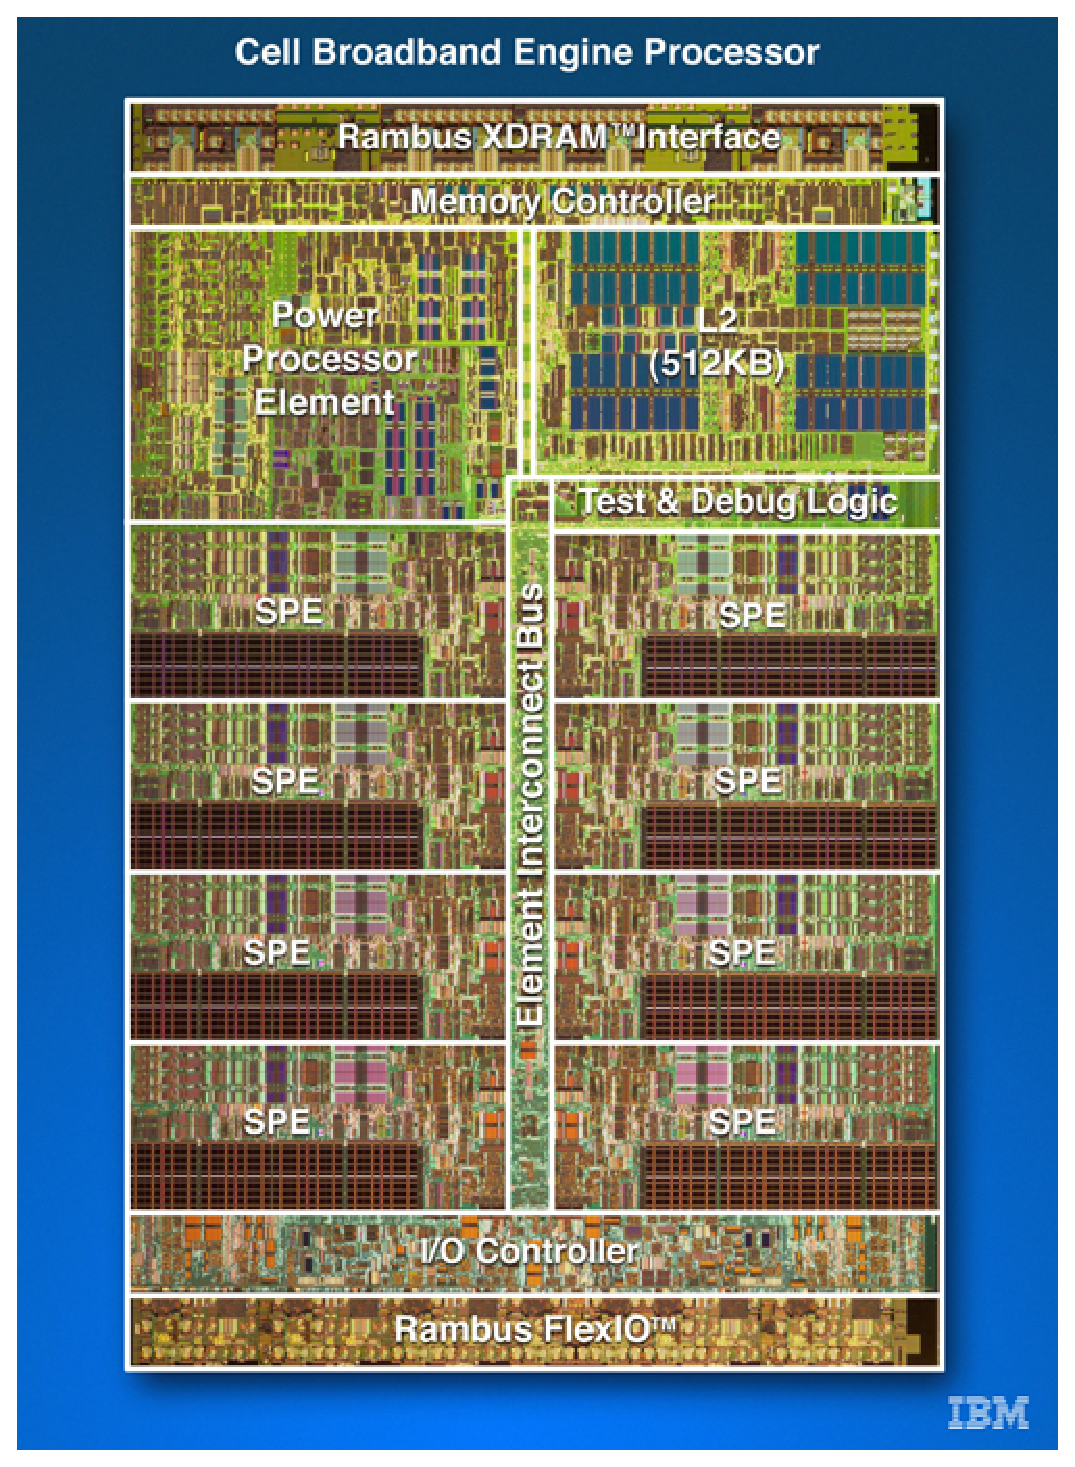
\includegraphics{cell}}
%    \caption{Cell Broadband Engine}
%    \label{image:cell}
%    \end{center}
%\end{figure}

The \emph{Cell Broadband Engine (Cell BE)}, developed jointly by Sony
Computer Entertainment, Toshiba, and IBM, is an (8+1)-way, 90nm SOI,
heterogeneous parallel processor that incorporates eight
\emph{synergistic processing elements (SPEs)} and one
\emph{power processing element (PPE)} connected via an
\emph{Element Interconnect Bus (EIB)}.  The EIB also connects
a memory controller (MIC) and two off-chip I/O interfaces.
This processor is used in the Sony Playstation 3 gaming console,
and is currently offered in products from IBM (QS21 blade)
and Mercury Computer Systems
(CAB PCI-e card and DCBB2 blade) \cite{mercury}.

The PPE is a modestly provisioned general purpose processor capable
of running the Linux OS, and which serves as a controller for
the eight SPEs.  It supports two execution threads and has a
theoretical peak performance of 6.4 Gflop/s double precision at 3.2 GHz.

Each SPE processor is a 128-bit vector engine with a 256 KB
user-controlled, embedded SRAM called the \emph{Local Store (LS)}.
Additionally, each SPE has a 128-bit, 128-entry register file.  All
data and text operated on by the SPE must be fetched from main
memory to the LS using \emph{direct memory access (DMA)} calls.
Each SPE has its own \emph{Memory Flow Controller (MFC)} that
supports up to 12 outstanding DMA requests and has a theoretical
bandwidth of 25.6 GB/s to main memory using DDR2-800
SDRAM\footnote{The current plan of record for RoadRunner
calls for DDR2-667, in which case, the theoretical bandwidth
will be 21.4 GB/s.}.  SPEs support dual-issue on even and odd
execution pipelines and have a theoretical single-precision,
peak performance of 204.8 Gflop/s at 3.2 GHz.  Double-precision
computation is possible on the Cell BE, although at the much
lower rate of $\sim$14.63 Gflop/s at 3.2 GHz.

The EIB is configured as a four-way, circular ring with paired
counter-rotating, uni-directional channels that are each
16 bytes wide.  There are currently 12 units connected to
this bus, so that the maximum number of steps between any two
units is six.  Each SPE has a 16 byte read port and a 16 byte
write port, and is capable of performing a read or write of 16
bytes on every EIB clock cycle.  SPEs are able overlap
computation with communication using special DMA queues for
requests that are still in flight.  The EIB operates at one-half
the system clock speed and has an aggregate theoretical
bandwidth of 204.8 GB/s at 3.2 GHz.

\subsection*{IBM PowerXCell 8I (eDP)}

IBM has developed an enhanced version of the Cell BE chip
specifically designed for use in supercomputing.  This chip,
the IBM PowerXCell 8I, adds fully-pipelined, double-precision
computing capability to the SPEs of the Cell BE chip.
The PowerXCell 8I uses a 65nm SOI process and has a
double-precision theoretical peak performance of 102.4
Gflop/s at 3.2 GHz.  Except as regards double-precision
performance, the PowerXCell 8I does not differ significantly
from the Cell BE.  This is the Cell chip that is used in RoadRunner.

%%%%%%%%%%%%%%%%%%%%%%%%%%%%%%%%%%%%%%%%%%%%%%%%%%%%%%%%%%%%%%%%%%%%%%%%%%%%%%%%
% Early Hardware Access
%%%%%%%%%%%%%%%%%%%%%%%%%%%%%%%%%%%%%%%%%%%%%%%%%%%%%%%%%%%%%%%%%%%%%%%%%%%%%%%%
\section*{Early Hardware Access}

As part of the RoadRunner deployment, two identical test systems
---both called ASDS-- are available to developers in preparation
for moving to the full machine.  Each of these has 12 Triblade
compute nodes and one I/O node, which are accessable through a
front-end using MOAB and Torque.  Disk access is available
through NFS.  With 12 Triblades, each test system has a total of
24 dual-core Opterons and 48 Cell eDP processors with a peak
theoretical performance of 4.9 Tflop/s\footnote{This is the
Cell-only performance.  The Opterons add another 172.8 Gflop/s.}
at 3.2 GHz.  Currently, these machines are not collocated,
and cannot be used as a single cluster.

Members of the Performance and Architecture Team (PAL) at
Los Alamos National Laboratory were given early access to a
CU at IBM's test facilities in Poughkeepsie, New York.  This system
was used to conduct some of the scalability analysis presented
in \S \ref{sec:performance}.

%%%%%%%%%%%%%%%%%%%%%%%%%%%%%%%%%%%%%%%%%%%%%%%%%%%%%%%%%%%%%%%%%%%%%%%%%%%%%%%%
% Science
%%%%%%%%%%%%%%%%%%%%%%%%%%%%%%%%%%%%%%%%%%%%%%%%%%%%%%%%%%%%%%%%%%%%%%%%%%%%%%%%
\section*{Laser Plasma Interaction in Inertial Confinement Fusion Experiments}

The multi-billion dollar National Ignition Facility (NIF) at 
Lawrence Livermore National Laboratory
is designed to reach conditions for ignition of thermonuclear fusion in a 
laser-driven inertial confinement fusion (ICF) capsule.  Achieving fusion ignition 
will be one of the landmark achievements in science and engineering and will
have a host of potential applications, including fusion energy research, 
high energy density physics, and laboratory astrophysics.  
In NIF ICF experiments, which commence in 2010, 192 laser beams with aggregate 
energy 1.8~MJ are directed onto the inner walls of a hohlraum, 
a roughly centimeter-sized cylindrical radiation ``bottle'' made of high-$Z$ material 
such as gold or uranium.  The walls heat up and radiate x-rays, which are absorbed 
by a tiny capsule
of cryogenic deuterium-tritium (DT) ``fuel'' surrounded by a plastic or beryllium 
ablator.  The capsule compresses to plasma density of order hundreds of g/cc and 
temperature in excess of 10~keV, conditions under which the DT fuel can ignite. 

Laser-plasma instabilities (LPI) jeopardize the success of fusion ignition on 
the NIF.  LPI occur as the laser travels through the plasma medium inside the hohlraum 
and scatters from (and amplifies) density irregularities.  This leads to 
parametric instabilities that scatter the laser light, reflect some of the laser 
energy out of the hohlraum, and create hot electrons that pre-heat the capsule 
and possibly prevent it from achieving sufficient density for fusion ignition 
to occur.  Laser-plasma instabilities (LPI) are a major concern, as they constitute 
half of the margin for uncertainty in ICF experimental design.\cite{}   The most 
pernicious LPI are stimulated Raman scattering (SRS) and stimulated Brillouin 
scattering (SBS), where the laser light scatters off electron or ion density 
fluctuations (waves), respectively.  

In NIF laser beams, random phase plates are used to break each beam into a collection 
of smaller laser ``speckles'' or hot spots.  The geometry of the speckles depends
on the properties of the beam, including wavelength and diffraction ($f$/\#), and the 
random phase plate.  With VPIC running on the full Roadrunner platform, we have the 
opportunity for the first time to simulate \abinitio\ LPI within a solitary laser 
speckle under NIF-like conditions and \textit{fully resolve} the kinetic 
wave-particle dynamics.  
This provides us a unique opportunity for understanding LPI 
that will translate into improved predictive modeling of ICF experiments and
mitigation of risk for NIF ignition. 

%%%%%%%%%%%%%%%%%%%%%%%%%%%%%%%%%%%%%%%%%%%%%%%%%%%%%%%%%%%%%%%%%%%%%%%%%%%%%%%%
% Science method
%
% BJA:  Still working on this.  Describe simulation we are doing.  
%
%%%%%%%%%%%%%%%%%%%%%%%%%%%%%%%%%%%%%%%%%%%%%%%%%%%%%%%%%%%%%%%%%%%%%%%%%%%%%%%%
\section*{Plasma Physics Simulations}

Under the range of laser and plasma conditions in ICF experiments, LPI evolve until 
they reach a complex, highly nonlinear state involving wave-wave coupling, 
wave-particle interaction, and trapping of plasma particles in waves.  Under the 
conditions of highest concern for ignition, wave-particle interactions dominate the 
nonlinearity. 
Understanding LPI under these conditions requires high-resolution kinetic plasma 
simulations, as afforded by the use of VPIC on Roadrunner, that capture all of the
wave-particle physics.  These simulations must resolve very complex particle orbits and
complicated structures in phase space and therefore require the use of many simulation 
macroparticles (as many as thousands of particles/cell of each species) to reach 
convergence of the dynamics.~\cite{}  

Recent experimental~\cite{} and modeling~\cite{} work shows that LPI
in a solitary laser speckle is represented well by a diffraction-limited laser beam.  
In our three-dimensional VPIC simulations, we launch a Gaussian diffraction-limited 
laser beam from the left simulation boundary into a plasma volume of dimension 
$35 \times 6 \times 6$~$\mu$m; the simulation boundaries absorb
electromagnetic waves and reflect particles.  
The $f/4$ beam is linearly polarized, of wavelength 
$\lambda_0 = 351$~nm,  
and has peak intensity ranging from $I_0 = 10^{15} - 10^{17}$~W/cm$^2$ at best 
focus, located at the center of the simulation volume.  The plasma is underdense 
with electron density $n_e = 0.14 n_{\mathrm{cr}}$; here 
$n_{\mathrm{cr}} = c m_e / 2 \lambda_0 e^2$ represents the critical 
density of the medium, $c$ is the speed of light in vacuum, $m_e$ is the electron
mass, and $e$ is the electronic charge in statcoulombs.  
We have chosen the simulation volume to span two Rayleigh lengths in the
the direction of laser propagation and three times the Gaussian width of the laser 
at the entrance plane.  The electron and ion temperatures are 
$T_e = 4$~keV and $T_i = 1$~keV respectively, which match hohlraum plasma conditions 
when the drive lasers are at highest intensity.  The hohlraum is filled with a plasma
comprising hydrogen, helium, and (possibly) trace amounts of krypton and xenon. 

The key dimensionless number characterizing LPI is $k \lde = 0.34$, where $k$ is 
the wavenumber of the most unstable SRS electron density fluctuation and 
$\lde = (k_B T_e / 4 \pi n_e e^2)^{1/2}$ is the Debye length ($k_B$ is Boltzmann's 
constant), the length scale above which 
the plasma dynamics are dominated by collective motion of the plasma as opposed to 
binary interactions among particles.  
The simulation time is $10000~\wpe^{-1}$ ($\wpe = (4 \pi n_e e^2 / m_e)^{1/2}$, which 
translates to $1.3 \times 10^5$ time steps.  This provides ample time for growth of the
first ``bursts'' of SRS as well as development of ion density structures (SBS).  
The simulation volume is divided evenly into cells with dimension 
$1.3 \times 1.7 \times 1.7$~Debye lengths, which ensures 15 cells in the longitudinal 
($x$) direction for resolving the most unstable electron density fluctuations and ample 
resolution (several tens of cells) for the transverse modes that develop.  

We have chosen this problem in order to resolve two outstanding questions in LPI 
physics:  (1) What is the role is of trapped particles in the nonlinear evolution of
SRS?  (2) What is the effect of adding trace amounts of high-$Z$ dopants to the 
hohlraum plasma environment?  

\textbf{Problem 1}
We verify 
recent work by the authors~\cite{} that shows both SRS and SBS saturate via nonlinear 
wave-particle trapping that bends electrostatic wavefronts and de-tunes the parametric 
coupling, followed by transverse filamentation and break-up of wave fronts.  
On Roadrunner, we run, for the first time, calculations of 1.1 trillion ($10^{12}$) 
simulation macroparticles, nearly a factor of six larger than the next largest PIC 
simulations of plasma~\cite{} (also with VPIC), to verify that the nonlinear processes 
we identify are indeed the ones that govern LPI saturation.  

\textbf{Problem 2}
We study the effects of adding high-$Z$ plasma components to the gas fill, a 
proposed LPI mitigation scheme~\cite{} and a problem arising for understanding of 
LPI near the hohlraum boundary (where gold and uranium plasma mix with the low-$Z$ gas) 
and ablator edge.  VPIC allows use of an aribitrary number of different plasma species, 
so it is ideal for these studies.  In this work, we use concentrations krypton and 
xenon of noble gases in addition to the hydrogen and helium gas fill.  To compare 
with small-scale laboratory experiments of LPI, we use a more diffracted beam ($f/3$) 
at higher intensity ($I_0 = 10^{17}$~W/cm$^2$). This problem requires very large numbers
of macroparticles/cell to resolve the ion kinetics; projected scaling of this problem 
on the full Roadrunner system approaches 400 TFlop/s.  

The early Roadrunner deployment lacks a high-performance file system, so our primary 
diagnostic for both studies is the integrated Poynting flux (scattered laser power) 
leaving the simulation volume, a quantity sampled every 16 time steps, that we compute 
and output with negligible computational, communications, or I/O overhead.  Based 
on a large body of verification and validation studies 
for VPIC LPI simulation~\cite{}, we have high confidence that single-precision studies 
are more than adequate. 


%%%%%%%%%%%%%%%%%%%%%%%%%%%%%%%%%%%%%%%%%%%%%%%%%%%%%%%%%%%%%%%%%%%%%%%%%%%%%%%%
% Numerical approach
%%%%%%%%%%%%%%%%%%%%%%%%%%%%%%%%%%%%%%%%%%%%%%%%%%%%%%%%%%%%%%%%%%%%%%%%%%%%%%%%
\section*{The VPIC Particle-In-Cell Code}

VPIC is a three-dimensional, relativistic, electromagnetic, particle-
in-cell code that has been highly optimized to minimize data movement, 
a predominate consideration that must be addressed for many codes in 
order to achieve high levels of performance on modern computing 
architectures.  As a part of this strategy, VPIC uses an 
asymptotically optimal sorting algorithm to re-arrange particle data, 
at a compile-time configurable rate, to maintain good spatial locality 
of memory access to particle data.  This approach also increases 
temporal locality of the field data accesses used to update particle 
positions and velocities.  Additionally, the data layouts and 
computational algorithms used by VPIC have been designed to take 
advantage of the short-vector, SIMD execution pipelines that are 
available on many modern processors.  These characteristics, combined 
with VPIC's effective use of single-precision floating-point 
computation --- a factor of two increase in the theoretical peak 
attainable on some architectures, and a factor of two decrease in data 
movement --, make it one of the highest performing particle-in-cell 
applications in existence.



% Cut/paste from Kevin's paper

\section{
II. VPIC Algorithms}

\subsection{A. PIC Overview}

VPIC integrates the relativistic Maxwell-Boltzmann equations in a linear background medium
\begin{eqnarray}
\PDeriv{f_s}{t} &+& 
\DotP{c\gamma^{-1}\vecu}{\Grad{f_s}} +
\DotP{\frac{q_s}{m_s c}\left(\vecE+\CrossP{c\gamma^{-1}\vecu}{\vecB}\right)}
{\Gradu{f_s}} = \left(\PDeriv{f_s}{t}\right)_{coll} \label{eq:Boltzmann}\\
\PDeriv{\vecB}{t} &=& -\Curl{\vecE} \label{eq:Faraday}\\
\PDeriv{\vecE}{t} &=&
\eps^{-1}\Curl{\mu^{-1}\vecB} - \eps^{-1}\vecJ - \eps^{-1}\sigma\vecE
\label{eq:Ampere}
.
\end{eqnarray}
Above, $f_s\left(\vecr,\vecu,t\right)$ is the smooth part of the
instantaneous phase-space distribution of a species $s$ with particle
charge $q_s$ and mass $m_s$.  $c$ is the speed of light in vacuum,
$\vecu$ is the normalized momentum and $\gamma\left(\vecu\right) =
\sqrt{1 + u^2}$ is the relativistic factor.
$\vecE\left(\vecr,t\right)$ and $\vecB\left(\vecr,t\right)$ are the
electric and magnetic field and $\vecJ\left(\vecr,t\right) =
\sum_s \int d\vecu q_s c\gamma^{-1}\vecu f_s$ is the current
density.  $\eps\left(\vecr\right)$, $\mu\left(\vecr\right)$ and
$\sigma\left(\vecr\right)$ are the background medium diagonal
permittivity, permeability and conductivity tensors.
$\left(\PDeriv{f_s}{t}\right)_{coll}$ represents discrete
particle effects (e.g. short range Coulomb collisions, excitation and
ionization).

Since a direct discretization of $f_s$ is prohibitive, PIC simulations
sample it with a collection of computational particles---each
computational particle typically represents many physical particles.
\eq{Boltzmann} is replaced by the computational particle
equations of motion
\begin{eqnarray}
\Deriv{r_{s,n}}{t} &=& c \gamma_{s,n}^{-1} \vecu_{s,n} \label{eq:Position}\\
\Deriv{u_{s,n}}{t} &=& \frac{q_s}{m_s c} \left[
\vecE\left(\vecr_{s,n},t\right) +
\CrossP{c\gamma_{s,n}^{-1}\vecu_{s,n}}{\vecB\left(\vecr_{s,n},t\right)}
\right] \label{eq:Momentum}
.
\end{eqnarray}
$f_s$ for the computational particles obeys \eq{Boltzmann} outside of
discrete particle collisional effects.  A smooth $\vecJ$ is computed
from the particle motion for use in \eq{Faraday}-\eq{Ampere}.  Because
$\vecJ$ is smooth, $\vecE$, $\vecB$ and $\vecJ$ can be sampled on a
mesh and interpolated between the mesh and particles.

PIC simulations of these equations can be distinguished by the time
stepping, field discretization, interpolation and collision methods.
VPIC uses state-of-the-art techniques, many of which are in use in
other codes
\cite{Kwan_Snell_1985,Verboncoeur_et_al_1995,Eastwood_et_al_1995,Jones_et_al_1996,Blahovec_et_al_2000,Nieter_Cary_2004}.
The methods are summarized below for completeness; more in-depth
analysis of PIC simulation can be found in
Refs.~\cite{Birdsall_Langdon_1985,Hockney_Eastwood_1988}.  For the
sake of brevity, collisional methods will not be discussed in this
paper.

\subsection{B. Time and space discretization}

The formal solution of $\Deriv{X}{t} = \op X$ for an operator $\op$ is
$X\left(\delta_t\right) = e^{\delta_t\op} X\left(0\right)$.  A second
order operator splitting \cite{McLachlan_Quispel_2002} for
\eq{Faraday}-\eq{Momentum} is
$e^{\delta_t\op_{ub}/2} e^{\delta_t\op_{ue}/2} e^{\delta_t\op_r/2}
e^{\delta_t\op_B/2}e^{\delta_t\op_E} e^{\delta_t\op_B/2}
e^{\delta_t\op_r/2} e^{\delta_t\op_{ue}/2} e^{\delta_t\op_{ub}/2}$,
where $\op_B$ is associated with \eq{Faraday}, $\op_E$ is associated
with \eq{Ampere}, $\op_r$ is associated with \eq{Position}, $\op_{ue}$
is associated with the electric force contribution to \eq{Momentum}
and $\op_{ub}$ is associated with the magnetic force contribution to
\eq{Momentum}.  Grouping the updates for $\vecE$ and $\vecB$ separately
from the others in the repeated application of this splitting and
noting the effect of $e^{\delta_t\op_r/2}$ is independent of $\vecE$
and $\vecB$ yields the well known velocity Verlet field advance,
$e^{\delta_t\op_B/2} e^{\delta_t\op_E} e^{\delta_t\op_B/2}$, and
leap-frog particle advance, $e^{\delta_t\op_r/2} I_J
e^{\delta_t\op_r/2} e^{\delta_t\op_{ue}/2} e^{\delta_t\op_{ub}}
e^{\delta_t\op_{ue}/2}$ ($I_J$ indicates that $\vecJ$ is computed for
the field advance but the state is unchanged) that advance
$\vecu_{s,n}$ from $t-\delta_t/2$ to $t+\delta_t/2$ and $\vecr_{s,n}$,
$\vecE$ and $\vecB$ from $t$ to $t+\delta_t$.

The simulation domain is divided into a regular mesh of identical
rectangular cells with potentially irregular but cell aligned
boundaries.  $\vecE$ and $\vecB$ are staggered; $E_x$ is sampled at
the middle of $x$-directed cell edges, $B_x$ is sampled at the middle
of $yz$-oriented cell faces and similarly for the $y$ and $z$
components.  $\vecJ$ is sampled the same as $\vecE$.  A variety of
particle and field boundary conditions are supported on the domain
boundaries including particle absorbing, particle reflecting, particle
refluxing, perfect electric conductor, perfect magnetic conductor,
field emitting and field absorbing (first order Higdon
\cite{Higdon_1986}).

\subsection{C. Particle advance}

In exact arithmetic, exactly applying $e^{\delta_t\op_r}$ is trivial,
$\vecr_{s,n} \leftarrow \vecr_{s,n} + \delta_t
c\gamma_{s,n}^{-1}\vecu_{s,n}$.  Applying $e^{\delta_t\op_{ue}}$ is
similarly trivial, $\vecu_{s,n}\leftarrow\vecu_{s,n} +
\frac{q_s\delta_t}{m_s c}\vecE\left(\vecr_{s,n},t\right)$.
Applying $e^{\delta_t\op_{ub}}$ is more involved, $\vecu_{s,n}
\leftarrow$ Rotate $\vecu_{s,n}$ around
$\vecB\left(\vecr_{s,n},t\right)$ by
$q_s\delta_t\left|\vecB\left(\vecr_{s,n},t\right)\right| /
\left(m_s\gamma_{s,n}\right)$ radians; this can be done efficiently
with a modified Boris push \cite{Boris_1970}.  To avoid aliasing of
cyclotron motion above the simulation Nyquist frequency if this done
exactly, VPIC uses a 6th order rotation angle approximation that is
also more efficient to compute.  The resulting update still conserves
energy like the exact update but will not non-physically couple high
frequency cyclotron motion to low frequency phenomena.  A similar
method is used in Ref.~\cite{Blahovec_et_al_2000}.

VPIC uses an energy conserving interpolation scheme for the particle
fields.  For example, $E_x$ is bilinearly interpolated from the four
$E_x$ edge samples and $B_x$ is linearly interpolated from two $B_x$
face samples of the cell containing a particle.  While this scheme
does not yield as smooth a field interpolation as a momentum
conserving trilinear interpolation, this interpolation is consistent
with a finite element time domain treatment of
\eq{Faraday}-\eq{Momentum} for this discretization
\cite{Eastwood_et_al_1995} and is easier to implement in simulations
with irregular boundary conditions as no resampling of field
components is required.

VPIC uses the charge conserving method of Villasenor and Buneman
\cite{Villasenor_Buneman_1992} to compute $\vecJ$ for the
field advance.  A particle makes a $\vecJ$ contribution in each cell
it passes through during a time step.  In exact arithmetic, the
resulting $\vecJ$ satisfies the discretized charge conservation
equation implicit in the field advance described below for a trilinear
$\rho$ accumulation.  Though this is often considered prohibitively
expensive, this eliminates issues that can arise from the build up of
Gauss' law violations.  Further, determining all the cells a particle
passed through provides efficient and robust particle boundary
interaction detection.

\subsection{D. Field advance}

Exactly applying $e^{\delta_t \op_B}$ is trivial, $\vecB \leftarrow
\vecB - \delta_t \Curl{\vecE}$.  Exactly applying
$e^{\delta_t \op_E}$ is more involved but can be done via
exponential differencing, $\vecE \leftarrow e^{-\delta_t \eps^{-1}
\sigma} \vecE +
\sigma^{-1}\left( 1 - e^{-\delta_t \eps^{-1} \sigma} \right)
\left( \Curl{\mu^{-1}\vecB} - \vecJ \right)$ (note that the second
term coefficient asymptotes to $\delta_t \eps^{-1}$ in the limit
$\sigma \rightarrow 0$).  The needed curls are computed with second
order accurate finite differencing.

A charge conserving $\vecJ$ and the above imply a discretized Gauss'
law.  However, in finite precision, arithmetic error can cause small
violations of this law to accumulate.  To accommodate, VPIC
periodically applies Marder passes \cite{Marder_1987} tuned
specifically to clean arithmetic error induced violations.  While this
method is local and inexpensive, it suffices to use it infrequently to
keep this law satisfied to near machine precision.

For wavelengths comparable to the cell dimensions, the discretized
speed of light can deviate significantly from $c$ and relativistic
particle motion can generate non-physical Cherenkov radiation at these
wavelengths.  To combat this, VPIC uses the transverse current
adjustment method discussed in Ref.~\cite{Eastwood_et_al_1995}.
Effectively, a computationally inexpensive current that obeys $\vecJ_T
= \tau \PDeriv{\left(\vecJ_T - \Curl{\mu^{-1}\vecB}\right)}{t}$ is
included that damps short wavelength radiation on a timescale $\tau$
while leaving the discretized charge conservation properties unchanged.

\subsection{E. Stability}

In vacuum, the field advance reduces to a basic FDTD algorithm
\cite{Yee_1966} and the time step and mesh spacing must satisfy the
Courant condition,
$\left(c\delta_t/\delta_x\right)^2 +
 \left(c\delta_t/\delta_y\right)^2 +
 \left(c\delta_t/\delta_z\right)^2 < 1$.
Additionally, the particle advance usually requires the time step and
cell dimensions to satisfy $\omega_p \delta_t < 2$ and $\delta_{x,y,z}
\approx \lambda_d$ where $\omega_p$ is the peak plasma frequency and
$\lambda_d$ is the plasma Debye length
\cite{Birdsall_Langdon_1985,Hockney_Eastwood_1988}.
Given particles cannot exceed $c$, satisfying the Courant condition
and the Debye criterion typically implicitly satisfy the plasma
frequency criterion.  Though the time step is stable for any cyclotron
frequency, it is usually desirable to resolve it to keep dynamics
accurate.  Also, sampling $f_s$ typically requires between tens and
thousands of particles per cell depending on the above parameters and
phenomena being studied to avoid non-physical computational particle
collisional effects.

\section{III. VPIC Implementation}

\subsection{A. Performance guidelines and optimization regime}

\begin{table}
\caption{\label{tbl:Rules_of_thumb}
VPIC implementation rules of thumb.  Data access estimates the time to
initiate a data transfer between the processor and a level in its
memory hierarchy.  Data movement estimates the time to move the next
32-bits in a transfer.  Internode figures were obtained from
benchmarks of typical high performance cluster interconnects.  The
single precision figure corresponds to a 2.5 GHz processor completing
a 4-vector SIMD instruction every clock.  Other rules of thumb were
similarly extrapolated from various data sheets and benchmarks.
Similar rules of thumb were applied in Ref.~\cite{Bowers_et_al_2006}.}

\begin{center}
\begin{tabular}{l l l c c c c}
\hline
\hline
\multicolumn{3}{c}{Operation} & \hspace{18pt} & Time & \hspace{18pt} & Rel.~Cost \\
\hline
Data access      & \hspace{9pt} & Internode & & 10 $\mu$s & & 100,000 \\
(Latency)        & & Memory    & & 50 ns     & & 500     \\
                 & & L2 Cache  & & 5.0 ns    & & 50      \\
\vspace{4pt}     & & L1 Cache  & & 1.0 ns    & & 10      \\
Data movement    & & Internode & & 5.0 ns    & & 50      \\
(32-bit)         & & Memory    & & 0.5 ns    & & 5       \\
                 & & L2 Cache  & & 0.2 ns    & & 2       \\
\vspace{4pt}     & & L1 Cache  & & 0.1 ns    & & 1       \\
Single precision & & FLOP      & & 0.1 ns    & & 1       \\
\hline
\hline
\end{tabular}
\end{center}
\end{table}

Most modern supercomputers consist of a large number of parallel
processing nodes connected by network.  The nodes themselves contain
one or more processors and memory.  Processor performance has improved
more rapidly than memory performance over recent decades.  To
compensate, modern processors use a deep memory hierarchy with faster
(though smaller and more limited) ``cache'' memories located close to
the processor.  Approximate rules of thumb for the cost of various
operations on processing nodes are given in \tbl{Rules_of_thumb}.
Achieving high performance requires minimizing latency, bandwidth and
computation, in roughly that order.  As physical constraints (such as
$c$) are already a noticeable component in many costs, the ratio
between processor and memory performance (particularly latency) should
not be expected to improve significantly in the future.

Fortunately, in most parallel relativistic codes, data needed for
computations on a node are spatially localized to that node or very
nearby; internode latency and bandwidth are naturally optimized.  For
example, in particle dominated simulations, VPIC has smoothly scaled
to some of the largest machines available (several thousand nodes)
without any special tuning effort when the simulation domain could be
statically decomposed to yield an approximately uniform number of
particles per node (even some highly non-uniform plasmas can be so
decomposed, especially if using variable particle charges).

Accordingly, in VPIC, local data motion is the dominant concern.
Unfortunately, on most processors, programmers have no control over
cache.  Rather, a processor heuristically caches data it anticipates
will be used.  Given this and \tbl{Rules_of_thumb}, minimizing local
data motion requires grouping data needed to perform critical
operations contiguously and accessing it sequentially when possible.
As computation and storage are virtually free compared to data motion,
replicating computations and/or data is often worthwhile.

In 3D PIC simulations, there tend to be many particles per cell on
average and more field and particle data per node than can fit in any
cache on that node.  In such a simulation, computation time is heavily
dominated by the particle advance.  VPIC is designed for this regime.
For the sake of brevity, only particle advance implementation
considerations are given and, unless otherwise stated, simulations
will be assumed to be in this regime.

\subsection{B. Single precision}

Single precision implementations can be made to run significantly
faster than their double precision counterparts as most modern
processors provide 4-vector single precision SIMD capabilities and
single precision requires half the data movement as double precision.
For typical time steps, cell dimensions and particles per cell,
discretization error exceeds single precision arithmetic error.  Thus,
single precision should be acceptable for such simulations provided it
does not introduce non-physical artifacts (e.g. large violations of
otherwise conserved quantities during the simulation).  VPIC uses
single precision to help achieve high performance but takes care to
structure operations to minimize its impact; some cases are discussed
below.

Unfortunately, languages like C and FORTRAN are not expressive enough
(e.g. data alignment restrictions) to allow compilers to use 4-vector
SIMD in operations as complex as those in VPIC.  To compensate, VPIC
has a C language extension that allows portable 4-vector SIMD code to
be written and converted automatically to high performance 4-vector
SIMD instructions on a wide variety of platforms.  A similar approach
was used in Ref.~\cite{Bowers_et_al_2006}.

A full discussion of single precision issues is beyond the scope of
this paper.  For examples of single precision use in applications with
far more demanding precision requirements, see
Ref.~\cite{Bowers_et_al_2006,Lippert_et_al_2007}.

\subsection{C. Single pass processing and particle data layout}

Since there is more particle data than can fit in any cache, it is
desirable to limit the number of times a particle is touched during a
time step lest performance be limited by moving particle data to and
from memory.  This can be achieved by processing the majority of the
particles in a single pass.  This, combined with the particle advance,
yields VPIC's inner loop structure:
\begin{verbatim}
for each particle
  interpolate fields
  update momentum
  update position
  accumulate current
end for
\end{verbatim}

To further minimize the cost of moving particle data, particle data is
stored contiguously, memory aligned and organized for 4-vector SIMD.
A particle looks like:
\begin{verbatim}
struct { float dx, dy, dz; int i;
         float ux, uy, uz; float q; }
\end{verbatim}
As a result, the inner loop streams through particle data once using
large aligned memory transfers under the hood---the ideal memory
access pattern.

\subsection{D. Field interpolation and particle sorting}

Field interpolation can severely impact performance if the data
choreography is not considered.  For example, if particles are stored
in a random order relative to the cells, mesh fields will be accessed
in a random order by the inner loop.  Because there is more mesh field
data than can be cached, these accesses will often require memory
transfers.  The situation is made worse if mesh fields are directly
accessed as several memory transfers may be necessary to load
non-contiguous field data.  Worse still if the field components are
stored in separate arrays.  In this worst case, VPIC's field
interpolation could involve up to 13 memory transfers per particle
under the hood (assuming adjacent $x$ data is contiguous in memory, 4
for $E_x$, 2 for $E_y$, $E_z$, $B_y$ and $B_z$ and 1 for $B_x$).
Further exacerbating this, far more data than requested would be
transfered; modern cores round-up the amount of memory transfered in
small requests like this to, at least, the (larger) memory-core dath
path width.

To make field interpolation efficient, an array of interpolation
coefficients is precomputed and saved in a contiguous, aligned,
4-vector SIMD compatible layout:
\begin{verbatim}
struct { float ex, dex_dy, dex_dz, d2ex_dydz;
         float ey, dey_dz, dey_dx, d2ey_dzdx;
         float ez, dez_dx, dez_dy, d2ez_dxdy;
         float bx, dbx_dx, by,     dby_dy;
         float bz, dbz_dz, pad0,   pad1;      }
\end{verbatim}
Additionally, the particle array is periodically sorted by the
containing cell index.  Because the particles do not move far per time
step, sorting is infrequent---every tens to hundreds of time steps.
Nevertheless, the sorting can be done efficiently in $O(N)$ operations
\cite{Bowers_2001}.

As a result, all the particles in a given cell are processed
approximately sequentially and the interpolation coefficients
necessary for these particles can be loaded once from memory and then
cached.  The interpolation coefficients themselves are accessed
approximately sequentially in large aligned transfers a near minimal
number of times.  Even though storing the interpolation coefficients
requires over three times as much memory as the mesh field data, the
net impact is to reduce memory transfers to minimal levels by making
more efficient use of cache.

Note that this approach generalizes to other interpolation strategies
(e.g. trilinear momentum conserving interpolation).  Likewise, already
having the particles sorted allows various particle-particle
collision models to be implemented more efficiently.  

This field interpolation approach is less effective when there are
very few particles per cell on average or when a large fraction of the
cells are devoid of particles.  In these cases, the field
interpolation coefficient computation time is not compensated by a
reduction in the particle field interpolation time.  However, given
that the cost of forming unused coefficients is small and that cells
containing multiple particles still see some benefit, this effect is
mild.  Further, this regime is atypical; sampling of $f_s$ well
typically requires many particles per cell on average.

High temperature particle distributions generally require more
frequent sorting to maximize overall performance than cold particle
distributions.  Fortunately, the finite speed of light in relativistic
simulation (or, more generally, timestep limitations due to numerical
aliasing instabilities induced by particles moving through too many
cells in a step) limit the rate at which the particle array becomes
disorganized at even the highest temperatures.  Interestingly,
non-thermal particle distributions (for example, fast moving cold
drifting particle beams) tend to need less performance sorting; as
these stay more organized physically, they stay more organized in
memory as well.  Also, the frequent sorting that occurs when using
various particle-particle collision models usually eliminates the need
for additional performance sorting.

\subsection{E. Position representation}

Positions are given by the containing cell index and the offset from
the cell center, normalized to the cell dimensions.  Having the index
makes determining which interpolation coefficients to load trivial.
The interpolation computation and current accumulation are likewise
very efficient as the particle offsets can be used directly.

This representation is also critical in single precision.  When an
absolute position representation is used, some coordinate information
encodes the containing cell index.  Thus, there is less information
available to encode the offset.  Consider a 1d simulation with $2^{10}
= 1024$ cells over the region $(0,1)$.  In single precision absolute
coordinates, particles in cell $0$ see a worst case absolute position
resolution of $2^{-24}/2^{10} \sim 5.8e-11$ while particles in cells
$512-1023$ see a resolution of $2^{-24} \sim 6.0e-8$.  In index plus
offset representation, all particles see a resolution of
$2^{-25}/2^{10} \sim 2.9e-11$ (the sign bit provides one bit of
position resolution) regardless which cell contains them.  This is
better everywhere than the absolute representation and does not
exhibit numerical anisotropy.  Interestingly, VPIC has identical
numerical properties for each cell regardless how the cell mesh is
translated, oriented or reflected in absolute coordinates.

This representation requires that the coordinate system for the
particle offsets need to be transformed when a particle crosses into a
different cell.  This cost is trivial and can be elegantly
incorporated into the charge conserving current accumulation.
Additionally, this representation generalizes naturally to more
advanced PIC algorithms (e.g. boundary fitted curvilinear meshes).

\subsection{F. SIMD, current accumulation and exceptions}

Given the single precision usage and SIMD compatible data layouts, all
particle processing described above is ideal for 4-vector SIMD.
Unfortunately, current accumulation is not.  Determining the cells
through which a particle passed varies from particle to particle; one
particle might remain in the cell in which it started while the next
might cross through several.  To utilize 4-vector SIMD, VPIC exploits
that particles do not cross cell boundaries often.  Consider a fairly
extreme simulation with a uniform isotropic light species
(e.g. electrons) with $\omega_p \delta_t \sim 0.2$ and $\delta_x \sim
\lambda_d$ (by the Courant condition, the thermal velocity would be
$\sim 0.1c$) and a heavy species (e.g. hydrogen) at the same
temperature.  Only $\sim 41\%$ of light species particles and $\sim
1.1\%$ of heavy species particles will cross a cell boundary in a time
step.  VPIC advances 4 particles at a time with 4-vector SIMD by
assuming none of the 4 particles cross cell boundaries.  Particles
that do cross are detected and make zero current contribution during
this process.  These particles are processed in scalar code
subsequently.

Other particle distributions may have different performance
characteristics, but, as noted above, simulation stability criteria
(especially in 3D) generally limit the number of cell boundaries a
particle will cross in a timestep to a few with most not crossing at
all.  Further, in many simulations with a drifting particle species,
the simulation frame can be chosen to reduce such potential
performance impacts---this can even improve numerical quality and
yield significantly less stringent simulation stability criteria
\cite{Vay_2007}.

Like the interpolation coefficients, current contributions from
particle motion in a cell are made to a contiguous aligned set of
partial currents which is then postprocessed into $\vecJ$ prior to the
field advance.  The same benefits as described for interpolation
coefficients apply here.

During cell crossing current accumulation, if a particle hits an
``exceptional'' boundary (e.g. needs communication to neighbor node,
needs absorbed, needs refluxed, ...), the index and remaining particle
displacement are saved to an exception list for later processing.
This has several benefits: no additional passes through the particles
are necessary to find exceptions, exception handling (often slow and
application specific) is cleanly separated from the high performance
general particle advance and exception handling does not pollute the
instruction or data caches while the particle advance is running.
Exception processing itself does not use any dramatic techniques.  In
3D, exception processing time typically scales as the simulation
domain surface area (and any boundaries within that domain); this is
negligible compared to the particle advance time which scales as the
simulation domain volume.

\subsection{G. IBM Cell Considerations for Roadrunner}

VPIC was recently ported to IBM's Cell processor.  Each Cell processor
contains one general purpose core and eight high performance 4-vector
SIMD processor cores (``SPE'').  Each SPE can only directly access 256
KB of high performance memory specific to it.  This ``local store'' is
analogous to cache, but, unlike conventional cache, memory transfers
to and from it must be explicitly managed.  Though non-trivial, this
makes it possible to design high performance application specific
cache protocols. \cite{Kahle_et_al_2005}

On the SPEs, particle data is tripled buffered in blocks of $N=512$;
while a block is processed, the next is loaded and the previous is
stored.  An $N$ line software cache of read-only interpolation
coefficients and read-write partially accumulated currents handles
inner loop random memory access.  It has a fully associative least
recently used policy (i.e. a line can hold any cell's data and the
least recently used line is replaced when caching new data); the last
$N$ distinct requests are guaranteed to be cached.  Before processing
a block, requests are made for all cells referenced in the block.
Most of these will already be in the cache.  Non-redundant memory
transfers are initiated for the remainder and block processing begins.
The net impact is minimal memory transfers are used, memory transfers
are overlapped with computation and the inner loop operates
exclusively out of cache (cell crossing current accumulation makes
additional requests following the inner loop).

While such a cache may seem expensive, each SPE can be faster (even
clock-for-clock) than a conventional processor core at cold particle
advances.  Presently, VPIC performs at $\sim 173$ million cold
particles advanced per second on a 3.2 GHz Cell ($\sim 49\%$ of
measured peak memory bandwidth and $\sim 21\%$ of theoretical
aggregate SPE single precision floating point performance).  By
comparison, VPIC runs at $\sim 12.6$ million PA/s on a single core 2.2
GHz AMD Opteron (used in the systems that ran the below examples).  As
Los Alamos's Roadrunner supercomputer plans to use $\sim 13,000$ Cell
eDP processors, a sustained rate up to $\sim 2.25$ trillion PA/s could
be achieved in particle dominated simulations.  As a cold particle
advance takes $\sim 246$ FLOP per particle (warm particle advances
take more, depending on simulation details such as temperature, for
cell crossing current accumulation), this is equivalent to $\sim
0.556$ quadrillion FLOP per second.

%%%%%%%%%%%%%%%%%%%%%%%%%%%%%%%%%%%%%%%%%%%%%%%%%%%%%%%%%%%%%%%%%%%%%%%%%%%%%%%%
% Moving the code to RoadRunner
%%%%%%%%%%%%%%%%%%%%%%%%%%%%%%%%%%%%%%%%%%%%%%%%%%%%%%%%%%%%%%%%%%%%%%%%%%%%%%%%
\section*{Adapting VPIC to RoadRunner}

In VPIC, performance is asymptotically limited by the rate particles
can be streamed to and from DRAM.  On Roadrunner, the bandwidth
between the Cell CPU and Cell local DRAM exceeds the bandwidth between
the Cell CPU and Opteron local DRAM (limited by the PCI-Express
bridge).  However, the Cell CPU to Cell CPU bandwidth is limited by
the internode Infiniband connection.  Accordingly, in porting VPIC to
Roadrunner, we decided (1) all local simulation state would reside
within Cell DRAM, (2) the Cell CPU would be responsible for all
simulation computations and (3) the Opteron cores would manage
communications between Cell CPUs.  This maximizes the bandwidth
between Cell CPUs and simulation state.  It also is less complicated
to implement and allows the VPIC to be used on Cell-only clusters.

% FIXME: BETTER QUANTIFY BANDWIDTH ABOVE?

%A kernel ported to the Cell SPE cores can have outstanding
%performance.  For example, in VPIC on Roadrunner, a SPE core is
%clock-for-clock faster than an Opteron core at the common case
%particle advance kernel ($158$ versus $174$ clocks per particle).
%Further the SPE cores run at a higher clock rate ($3.2 GHz$ versus
%$1.8 GHz$) and there are $8$ times as many of them.  As a result,
%VPIC's SPE accelerated particle advance kernel itself can achieve
%$0.517 Pflop/s$ on whole of Roadrunner, over $15$ times faster than
%the $0.033 Pflop/s$ can achieve by running the particle advance kernel
%on the Opteron cores.  (For reference, this corresponds to achieving
%$20\%$ of theoretical single precision peak performance on a Cell SPE
%core.)

%At the same time, a Cell PPE core is significantly less powerful than
%an Opteron core on Roadrunner.  Even though the parts of VPIC that run
%on the SPE cores run over an order of magnitude faster than if they
%were run on the Opteron cores in aggregate, the parts of VPIC that run
%on the PPE cores execute $\sim 2$ to $\sim 3$ times slower!  The
%typical overall simulation speed up achieved by porting VPIC from
%Roadrunner's Opterons to Roadrunner's Cells is a lower (though still
%impressive) $\sim 4$ to $\sim 8$, depending on simulation physical and
%numerical parameters.

% FIXME: BETTER QUANTIFY ON ASDS ABOVE?

%Thus, maximizing performance of a code like VPIC on Cell requires an
%all-of-nothing approach to porting.  In addition to SPE accelerating
%the dominant computational kernel, minor computations also need to be
%SPE accelerated lest they become performance bottlenecks.  Likewise,
%performance on Cell is much more sensitive to physical and numerical
%paraemters that affect these other computations.  In VPIC, though the
%infrequent particle sort, the field solve and the particle exception
%processing are typically negligible expenses when run on conventional
%clusters, they are large expenses (even dominant in some regimes)
%currently when VPIC is run SPE accelerated on Roadrunner.  Current
%VPIC development is focused on porting these operations to the SPE as
%well.

% FIXME: IN USE VOXEL TERMINOLOGY TO DISAMBIGUATE FROM CELL PROCESSOR
% IN TEXT OVERALL

Each Cell CPU contains $1$ general purpose core (``PPE'') and $8$ high
performance $4$-vector SIMD cores (``SPE'').  Each SPE can only
directly access $256$ KiB of high performance memory local to it.
This ``local store'' is analogous to cache, but, unlike conventional
cache, memory transfers to and from it must be explicitly managed via
the SPE's $32$ channel DMA engine.  Though non-trivial, this makes it
possible to design high performance application specific cache
protocols. % FIXME: CITE KAHLE_ET_AL_2005 HERE?

To process a particle list, the SPEs are assigned appromixately equally
sized non overlapping segments of the list and their own
current accumulator.  Each segment contains a
multiple of $16$ particles; the PPE advances any left overs while the
SPEs are working.  Particle data is triple buffered on the SPEs in
blocks of up to $512$ particles (at most $16$ KiB are needed to hold a
block---the largest size a single DMA transfer supports).
While a block is processed, the next is loaded and the previous is
stored.  $48$ KiB of local store and $3$ channels are used for particle
triple buffering.

Block processing groups particles by $4$ and uses $4$-vector SIMD to
advance them data parallel (much like is done on conventional
clusters).  To fully utilize the SPE's $128$ registers and minimize
pipeline stalls, the 4-vector inner loop is hand unrolled and modulo
scheduled by $4$.  Since a block is guaranteed to contain a multiple
of $16$ particles, no code is needed to process left
over particles.

The challenges of SPE particle processing are handling random
memory access and particle exceptions.  A $512$ line
software cache of read-only interpolation coefficients, read-only
voxel adjacencies and read-write partially accumulated currents
handles random memory access.  The cache has a fully associative
least recently used (LRU) policy; a line can hold any voxel's data and
the least recently used line is replaced when caching new data.

The cache has a simple interface:
\begin{verbatim}
  cache_line = voxel_cache_fetch( voxel_index )
\end{verbatim}
and:
\begin{verbatim}
  voxel_cache_wait()
\end{verbatim}

voxel\_cache\_fetch() initiates DMA transfers to evict the least
recently used cache line and replace it with the requested data.
voxel\_cache\_wait() waits until all pending cache DMA transfers are
complete.  Because the cache is LRU, it is easy to determine which
requests are still cached; the last $512$ unique requests are
guaranteed to be cached after a call to voxel\_cache\_wait() and before
any further calls to voxel\_cache\_fetch().  Accordingly, before processing
a block, voxel\_cache\_fetch() is called for each voxel referenced in
the block followed by a call to voxel\_cache\_wait().  Because the
particle list is approximately sorted at all times, most of these will
be cache hits.  Regardless, the cache is large enough that, even if
every particle in a block were in different voxels, all voxel data is
guaranteed to be in cache once block processing begins.

Under the hood, voxel\_cache\_fetch() queries a hash table to determine
if the requested voxel is already cached.  This hash table is
oversized to reduce collisions and uses linear probing and modular
hashing for implementation efficiency.  If a cache hit, the cache line
replacement order (stored as a doubly linked circular queue) is
updated.  If a cache miss, the least recently used line is selected
for replacement.  For read-only data, a DMA load on a channel selected
round robin from a set of channels reserved for this purpose is
initiated.  This allows multiple simultaneous fetches of read only
data.

Allowing multiple simultaneous fetches of read-write data is more
complicated as transfers to a given voxel must not be reordered by the
DMA engine.  For read-write data, if the line to fill needs
eviction first, a channel is selected based on the voxel index of the data
to evict, that data is copied to that channel's writeback buffer
(first waiting until any previous writebacks on that channel are
complete) and a DMA store is performed.  Then a fenced DMA load is
initiated for the requested read-write data on a channel selected
based on the requested voxel index.  Since all transfers of read/write
data to a given voxel use the same channel, the fence is effective.

Finally, the hash table and least recently used line are updated.
Though complicated, all operations above are a fast $O(1)$ on average.
A cache line requires $268$ bytes per line ($192$ for the actual data,
$4$ for the cache tag, $8$ for the LRU ordering and $64$ for the hash
table) and thus requires of $134 KiB$ local store.  $10$ channels are
reserved for transfers of read-only data and $16$ channels are
reserved for transfers of read-write data.  While such a cache may
seem expensive, a SPE core can be faster (even clock-for-clock) than a
conventional processor core at particle advances.  The net impact is
minimal DMA transfers are used, most DMA transfers are overlapped with
computation and the inner loop operates exclusively out of local store.

When a particle exception occurs that the SPE logic cannot handle
(e.g. particle needs communication to a neighboring node), the
particle's index and remaining displacement ($16$ bytes) is saved to a
list of exceptions that occured during block processing.  When
the processed block is stored, the list of unprocessed
exceptions that occured during is also streamed out to memory for
later processing.  Since up to $512$ exceptions could occur while
processing a particle block and there $3$ such blocks, $24
KiB$ of local store and $3$ DMA channels are used for managing
unprocessed exceptions.

Overall, $206$ KiB of local store data is used for particle
processing (leaving $56$ KiB for code) and all $32$ DMA channels
are utilized.

\subsection*{Message Passing Relay}

As mentioned earlier, as part of the adaptation of VPIC to the
Roadrunner architecture, we developed a message relay layer
called \emph{MP Relay}
that runs on the Opterons and handles forwarding
of message traffic and remote I/O operations for the diskless
QS22 blades (required for restart and visualizaiton dumps).
The original VPIC code already abstracted message passing
operations, so this modification was straightforward.

The MP Relay essentially flattens the hierarchical topology of
Roadrunner making it possible to use the same underlying
VPIC implementation to run on Roadrunner, clusters of Cell processors,
and traditional clusters with very few architecture specific code 
sections.  VPIC uses an autoconf-based build system, which supports
compile-time selection of the target architecture.  This allows
VPIC to easily be configured to use the original message passing
abstraction layer or the MP Relay.  The master control logic of the
code is unchanged.

Communication between Opterons and Cells is handled using the
\emph{Data, Communication, and Synchronization (DaCS)} library developed by
IBM.  This library provides send/recieve and put/get symmantics
for moving data over the PCI-e link between the LS21 and QS22 blades.
Communication between the Opteron host processes is implemented
using OpenMPI.

On the Operton side, the relay runs an event loop that issues
a non-blocking dacs\_recv call that accepts a point-to-point request
data structure from its associated PPE peer.
Incoming requests are passed through a switch statement
that makes additional non-blocking
send (dacs\_send) and recieve calls to complete the
point-to-point communication.  Messages that need to be
passed to other PPEs are sent via MPI calls to that PPE's host relay.
I/O requests are handled by double-buffered communication and
calls to fread and fwrite.

\begin{figure}
    \begin{center}
    \scalebox{0.25}{\input{relay.pstex_t}}
    \caption{MP Relay}
    \label{fig:relay}
    \end{center}
\end{figure}

%%%%%%%%%%%%%%%%%%%%%%%%%%%%%%%%%%%%%%%%%%%%%%%%%%%%%%%%%%%%%%%%%%%%%%%%%%%%%%%%
% Performance and Scalability
%%%%%%%%%%%%%%%%%%%%%%%%%%%%%%%%%%%%%%%%%%%%%%%%%%%%%%%%%%%%%%%%%%%%%%%%%%%%%%%%
\section*{Performance and Scalability} \label{sec:performance}

This section documents the methodologies used both in measuring actual performance on the currently available hardware, and in predicting the total performance that will be achieved on the full machine in June 2008.

\subsection{Operation Count}

The cycles in the calculation are dominated by the particle advance.
Within the particle advance, the most common case is a ``cold'' particle
advance, which means that the particle does not leave its cell.  Cold
particle advances require 246 operations:  60 additions, 80 multiplies, 1 
reciprocal (rcp),
2 reciprocal square roots (rsqrt), 6 compares, and 20 SIMD bit operations (logicals,
conditional moves, and conditional zeros).  The cost of a rcp 
(rsqrt) is assumed to be the initial approximation cost plus two additions and 
two (four) 
multiplies.  Taking the initial approximation cost of the rcp
and rsqrt to be four times the polishing cost (4 and 6 operations, respectively), and assuming that add, 
multiply, compare, and vector bit operations all cost one floating-point operation yields the total of 246 operations given above.

The non-common case involves a particle crossing a cell boundary.
Using similar estimates to those given for the rcp and rsqrt in the
``cold'' particle advance calculation, the non-common advance requires
an additional 168 operations: 52 additions, 29 multiplies, 3 reciprocals, 9 compares,
and 18 SIMD bit operations.

To estimate the total number of floating-point operations required to
push a single particle one step (for a given distribution and simulation
parameters in VPIC), a random distribution of $10^7$ thermal particles 
is created
and advanced for one iteration.  The resulting spatial distribution
is then analyzed to compute the probability that a particle will
cross a given number of boundaries.  The results of this approximation
are generally accurate to within 3 significant digits,
based on the assumptions that: 1) Particles are evenly distributed
in space, and 2) Particles have a drifting Maxwellian distribution.
Using this estimation with $\delta t = 0.02$ and cell
dimensions $1.3  \times 1.8 \times 1.8$ (in Debye lengths),
we obtain operation counts of 256.15 (for electrons,
using a thermal velocity $v_{\mathrm{th}} = 1.0$), and 246.25
(for ions, with thermal speed reduced by $(m_e/m_i)^{1/2}$)
are used in measuring the performance of VPIC.
These values are weighted by the fraction of the number of particles
of each type present
and averaged to obtain a single operation count.

This estimate represents a lower bound because we are not accounting
for cost of field solve or other bookkeeping. 

\subsection{Performance on a Single Cell Processor}

Two input decks,  P1 and P2, corresponding to the two problems 
identified above, were considered and used to evaluate the single-chip, 
PowerXCell 8I performance: 

\textbf{P1}:  On a single Cell processor, a $22 \times 21 \times 21$ mesh 
is used with 1755 particles/cell of each of five particle species.  
(This problem is 
more "common case'' 
in the ratio of particles/cell than P2).  
Scaled to the full Roadrunner machine, the simulation would 
use 1.1 trillion particles and 119 million cells.  This uses essentially
all available system memory (necessitating the use of an in-place sort). 
This problem systained 27.2 GFlop/s. 


\textbf{P2}:  On a single Cell processor, a $13 \times 14 \times 14$ mesh 
is used with 3900 particles/cell of each of five particle species.  
P2 showcases VPIC's ability to employ a very large number of particles/cell 
to resolve highly detailed phase space structures.  
Scaled to the full Roadrunner machine, this problem would employ 
643 billion particles and 33 million cells. This uses essentially
all available system memory, but with an out-of-place sort for improved 
sorting performance. 
This problem systained 32.2 GFlop/s. 

Performance is a balance between loss of spatial locality (which degrades
software cache performance on the SPU particle advance) and time spent
sorting particles.  Generally, electrons, being the hottest species, 
delocalize most rapidly and therefore need to be sorted more
frequently than the ions.  Careful steps were taken on both of these
problems to optimize electron/ion sorting intervals. 

\begin{table}
\caption{\label{tbl:ASDS_Weak_Scalability}
Weak Scalability}

\begin{center}
\begin{tabular}{l c c}
\hline
\hline
Cell Cores & Gflop/s per Core & Projected Full Machine Tflop/s Performance \\
 & & (based on this measurement) \\
\hline
1 & 32.2 & 404.3 \\
4 & 29.8 & 386.0 \\
8 & 29.1 & 377.5 \\
16 & 28.5 & 369.8 \\
36 & 28.4 & 367.5 \\
\hline
\end{tabular}
\end{center}
\end{table}

Outline I see (BJA):  
\begin{itemize}
\item XXXXX Single core performance on tuned VPIC deck.

\item ????? How we optimized:  large particle number; sort interval to be 
balance between performance gain from improved data locality vs. 
cost of doing the sort. 

\item ????? Breakdown of how we infer single-core performance.  (What flops go to 
what; worst-case, we give a lower bound on performance from cold particle
benchmark).  What does this translate into in terms of theoretical peak 
flops?  In terms of bandwidth to memory? 

\item Summarize Kevin Barker's measured scaling on a less-particle-dominated 
simulation.  (216 ppc on VPIC with broken earlier version of VPIC). 

\item Anticipated scaling for full Roadrunner from scaling up of tuned 
single-core measured performance (and as many as 48 cores of ASDS).  

\end{itemize}

%%%%%%%%%%%%%%%%%%%%%%%%%%%%%%%%%%%%%%%%%%%%%%%%%%%%%%%%%%%%%%%%%%%%%%%%%%%%%%%%
% Conclusion
%%%%%%%%%%%%%%%%%%%%%%%%%%%%%%%%%%%%%%%%%%%%%%%%%%%%%%%%%%%%%%%%%%%%%%%%%%%%%%%%
\section*{Conclusion}






%%%%%%%%%%%%%%%%%%%%%%%%%%%%%%%%%%%%%%%%%%%%%%%%%%%%%%%%%%%%%%%%%%%%%%%%%%%%%%%%
% biliography
%%%%%%%%%%%%%%%%%%%%%%%%%%%%%%%%%%%%%%%%%%%%%%%%%%%%%%%%%%%%%%%%%%%%%%%%%%%%%%%%
\begin{singlespace}
\bibliographystyle{plain}
\bibliography{bib/gb2008,bib/vpic}
\end{singlespace}

%%%%%%%%%%%%%%%%%%%%%%%%%%%%%%%%%%%%%%%%%%%%%%%%%%%%%%%%%%%%%%%%%%%%%%%%%%%%%%%%
% end document
%%%%%%%%%%%%%%%%%%%%%%%%%%%%%%%%%%%%%%%%%%%%%%%%%%%%%%%%%%%%%%%%%%%%%%%%%%%%%%%%
\end{document}
